\documentclass[tikz,border=6pt]{standalone}
\usepackage{xcolor}

\definecolor{blockblue}{HTML}{4A90D9}

\begin{document}
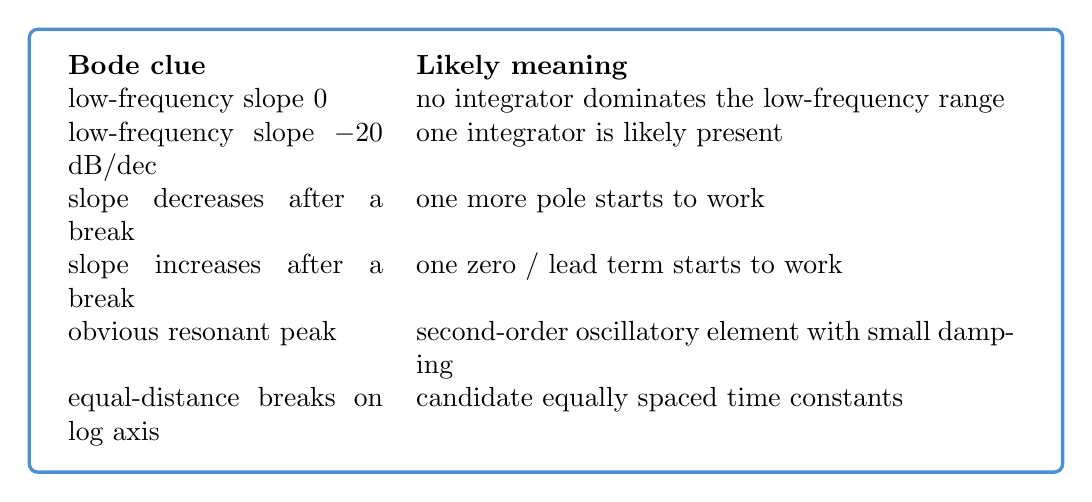
\begin{tikzpicture}[line width=1.2pt]
  \node[
    draw=blockblue,
    rounded corners=3pt,
    inner sep=8pt,
    align=left
  ] at (0,0) {
    \begin{tabular}{p{4.0cm}p{7.6cm}}
      \textbf{Bode clue} & \textbf{Likely meaning} \\
      low-frequency slope $0$ & no integrator dominates the low-frequency range \\
      low-frequency slope $-20$ dB/dec & one integrator is likely present \\
      slope decreases after a break & one more pole starts to work \\
      slope increases after a break & one zero / lead term starts to work \\
      obvious resonant peak & second-order oscillatory element with small damping \\
      equal-distance breaks on log axis & candidate equally spaced time constants \\
    \end{tabular}
  };
\end{tikzpicture}
\end{document}
